\documentclass[12]{article}

%% Set up in article mode
\usepackage{beamerarticle}
\setjobnamebeamerversion{tikzbox.beamer}

%% Set the paper geometry
\usepackage[a4paper, left=1.5cm, right=1.5cm, top=1.5cm, bottom=2.5cm]{geometry}

\usepackage[sc]{mathpazo}
\linespread{1.05}         % Palatino needs more leading (space between lines)
\usepackage[T1]{fontenc}

%% Listings hack
\usepackage{listings}
\lstset{
	basicstyle=\small,
	numbers=left,
	numberstyle=\tiny\color{gray},
	commentstyle=\itshape\color{blue},
}

%% Presentation Information
\title{Ticking the Ti\emph{k}Z Box}
\subtitle{Creating Diagrams with PGF/Ti\emph{k}Z}
\author{Andrew Mundy\\andrew.mundy@cs.man.ac.uk}
\date{}

%% TikZ
\usepackage{tikz}
\usetikzlibrary{automata,chains,scopes,patterns,petri}

%% etoolbox
\usepackage{etoolbox}

%% Subcaptions
\usepackage{subcaption}

%% Listings
\lstset{
	frame = tb,
	columns = fullflexible,
}

\begin{document}
	%% Document title
	\maketitle
	\begin{frame}
		\titlepage
	\end{frame}

	%% Grovel!
	I really hope that this document proves to be a useful reference; but am aware that it isn't as complete, or as well written, as I would desire!
	There are some pointers to better references on the last page.

	%% Include relevant sections
	\mode<all>
		\mode*		%% Reset Mode
\section{Getting Started}
\begin{frame}
	\frametitle{Installing Ti\emph{k}Z}

	Not necessary for \emph{new} TeXLive installs\ldots\\
	Sadly, this does not include School of CS Machines!

	\pause

	\begin{enumerate}
		\item Create a \texttt{texmf} directory
		\mode<article>
		\begin{itemize}
			\item \texttt{\$ mkdir \textasciitilde/texmf/}
		\end{itemize}
		\mode<all>

		\pause

		\item Download the PGF/Ti\emph{k}Z package
		\mode<article>
		\begin{itemize}
			\item Available from SourceForge \texttt{sourceforge.net/projects/pgf/}
		\end{itemize}
		\mode<all>

		\pause

		\item Extract the package in \texttt{\ldots/texmf/}

		\pause

		\item Run \texttt{texhash}
	\end{enumerate}
\end{frame}

\textit{Perhaps we should petition CSIS to get TikZ installed everywhere?}

\begin{frame}
	\frametitle{Using Ti\emph{k}Z}
	\begin{itemize}
		\item Include \texttt{\textbackslash usepackage\{tikz\}} in your \textit{preamble}
		\item Place Ti\emph{k}Z commands in the \texttt{tikzpicture} environment
	\end{itemize}
	\lstinputlisting[language=TeX]{examples.all/document.tex}
\end{frame}

\subsection{Drawing and Nodes}
\begin{frame}
	\frametitle{Drawing Primitives}
	Ti\emph{k}Z provides three drawing primitives:
	\begin{enumerate}
		\foreach \p in {path, draw, fill}{%
			\item \texttt{\textbackslash\p~[\textit{options}] \textit{co-ordinates};}
		}
	\end{enumerate}

	And three co-ordinate systems:
	\begin{description}
		\item[Cartesian] \texttt{(x \textit{units}, y \textit{units})}
		\item[Polar] \texttt{(angle in degrees:magnitude \textit{units})}
		\item[Named] \texttt{(predefined arbitrary name)}
	\end{description}
\end{frame}

This seems like the logical point to actually write some Ti\emph{k}Z, so we'll use each of the drawing primitives to draw a unit rectangle.
Along the way, we'll see what some of these mysterious options are.
The code used is shown in Listings \ref{listing.drawing-primitives.path}, \ref{listing.drawing-primitives.draw}, \ref{listing.drawing-primitives.fill};
and the results are in Figure \ref{figure.drawing-primitives}.

\begin{figure}[hb]
	\centering
	\foreach \primitive in {path, draw, fill}{%
		\begin{subfigure}{.25\textwidth}
			\centering
			\input{examples.article/drawing-primitives-\primitive}
			\caption{Drawing using ``\primitive''}
		\end{subfigure}
	}
	\caption{Using the TikZ drawing primitives to draw unit rectangles. Each primitive has its own unique quirks,
		and even though they are for the most part interchangeable, it's worth knowing what they are:
		namely, ``path'' will not display anything by default, so it can be quite useful for positioning nodes (more on this later);
		``fill'' will use the given colour to fill the area;
		and finally ``draw'' will use the given colour to stroke the area (I find I use this most).}
	\label{figure.drawing-primitives}
\end{figure}

\foreach \primitive in {path, draw, fill}{%
	\lstinputlisting[language=tex, caption={Using ``\primitive'' to draw}, label=listing.drawing-primitives.\primitive]%
		{examples.article/drawing-primitives-\primitive.tex}
}

\begin{frame}
	\frametitle{Shapes and Lines}
	We've seen the syntax for drawing rectangles, there's more\ldots
	\begin{description}
		\item[Rectangle] \texttt{rectangle (corner)} \tikz\draw [thick, red] rectangle (1em, 1em);
		\item[Circle] \texttt{circle [\textit{options}]} \tikz\draw [thick, blue] circle [radius=0.5em];
		\item[Ellipse] \texttt{ellipse [\textit{options}]} \tikz\draw [thick, purple] ellipse [x radius=.75em, y radius=.5em];
		\item[Curved Lines] \texttt{.. controls (-) and (-) ..}
			\tikz\draw [thick, green!50!black] (0,0)
				.. controls ++(0:0.5em) and ++(0:-0.5em) .. ++(1em, 1em)
				.. controls ++(270:.5em) and ++(0:-.5em) .. ++(.5em,-1em)
			;
		\item[Arcs] \texttt{arc [\textit{options}]} \tikz\draw [thick, gray] (0,0) arc [radius=1em, start angle=45, end angle=135];
	\end{description}
\end{frame}

Some further examples of these constructions are shown in Figure \ref{figure.drawing-primitives.shapes}, the code for which is shown in Listing \ref{listing.drawing-primitives.shapes}.

\begin{figure}[hbt]
	\centering
	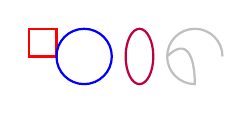
\begin{tikzpicture}
	%% Rectangle
	\draw [thick, red] (0,0) rectangle ++(1em, 1em);

	%% Circle
	\draw [thick, blue] (2em,0) circle [radius=1em];

	%% Ellipse
	\draw [thick, purple] (4em,0) ellipse [x radius=0.5em, y radius=1em];

	%% Curved Line linking into Arc
	\draw [thick, black!25!white] (5em,0)
		.. controls ++(45:1em) and ++(90:1em) ..
		++(1em,-1em) arc [start angle=270, end angle=0, radius=1em]
	;
	%% colour1!(0 <= x <= 100)!colour2 mixes colours by percentage
	%% i.e. black!25!white is 25% black, 75% white
\end{tikzpicture}

	\caption{Some more complicated constructions using TikZ drawing primitives.}
	\label{figure.drawing-primitives.shapes}
\end{figure}

\lstinputlisting[language=TeX, caption={More complicated shapes in TikZ}, label={listing.drawing-primitives.shapes}]{examples.article/drawing-primitives-shapes.tex}

\begin{frame}
	\frametitle{Nodes and Text}
	Amongst other things, nodes provide a way of adding text to a diagram.
	
	\texttt{\textbackslash node~\textit{at (...)} [\textit{options}] \textit{(name)} \{\textit{content}\};}

	\begin{center}
		\foreach \n in {1,...,4}{%
			\only<\n>{\input{examples.all/nodes-hello-\n}}
		}
	\end{center}

	\foreach \n in {1,...,4}{%
		\only<\n>{\lstinputlisting[language=tex]{examples.all/nodes-hello-\n.tex}}
	}

\end{frame}

\begin{frame}
	\frametitle{Nodes, Anchors and Co-ordinates}
	Nodes also provide our arbitrary co-ordinates/points.
	\begin{center}
		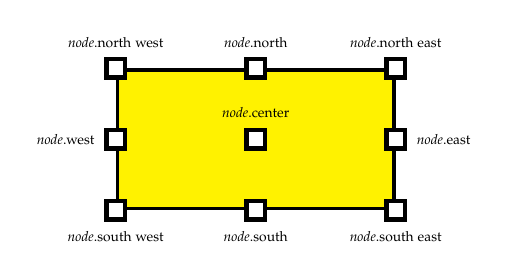
\begin{tikzpicture}[
	every label/.style = {font=\tiny},
]
	\node [minimum width=10em, minimum height=5em, draw, very thick, fill=yellow] (n1) {};

	\foreach \anchor/\labeldir in {west/left, north west/above, north/above, north east/above,
				       east/right, south east/below, south/below, south west/below, center/above}{%
		\node at (n1.\anchor) [label={\labeldir:{\textit{node}.\anchor}}, draw, ultra thick, fill=white] {};
	}
\end{tikzpicture}

	\end{center}
\end{frame}

We can put what we've got so far together in a fairly simple example.
Listing \ref{listing.nodes} shows the code for Figure \ref{figure.nodes}.

\begin{figure}[btp]
	\centering
	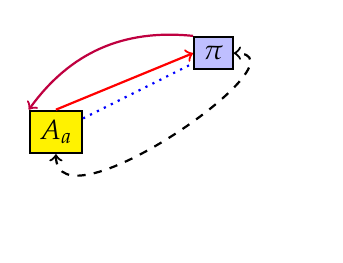
\begin{tikzpicture}
	%% Draw our two nodes -- note our content is mathematical
	\node at (0,0) [draw, thick, fill=yellow] (a) {$A_a$};		% Called `a'
	\node at (2,1) [draw, thick, fill=blue!25!white] (pi) {$\pi$};	% Called `pi'

	%% Connect up the node edges in various ways
	\draw [thick, dotted, blue] (a) -- (pi);	% Closest points
	\draw [thick, ->, red] (a.north) to (pi.west);	% `->' is an arrow
	\draw [thick, <->, dashed, out=-90, in=0] (a.south) to (pi.east); % Alternative bend mechanism
	\draw [thick, purple, bend left, <-] (a.north west) to (pi.north west);	% Yet another!
\end{tikzpicture}

	\caption{Uses of nodes and anchors; plus some additional options and semantic methods for constructing lines.}
	\label{figure.nodes}
\end{figure}

\lstinputlisting[language=TeX, caption={Combining nodes, anchors, and drawing.}, label={listing.nodes}]{examples.article/nodes-anchors.tex}

\mode<all>	%% Reset mode

		\mode*		%% Reset Mode

\section{A Worked Example}

\mode<presentation>
\begin{frame}
	\frametitle{Putting it all Together}
	Let's try to recreate this diagram:

	\begin{columns}[T]
		\begin{column}{.5\textwidth}
			\centering
			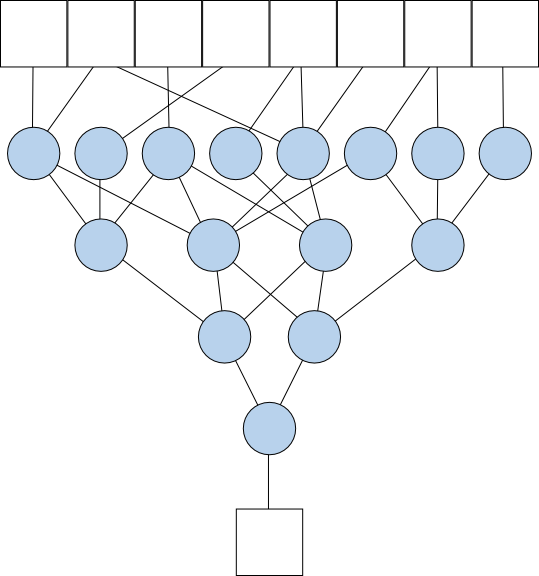
\includegraphics[width=\textwidth]{figures/specification}
		\end{column}
		\begin{column}{.5\textwidth}
			Assume structure is constant, but connections variable.

			How do we:
			\begin{itemize}
				\item \textbf{position nodes?}
				\item place edges?
			\end{itemize}
		\end{column}
	\end{columns}
\end{frame}
\mode*

We should now be able to put everything we've learnt together to develop a more complex example.
Specifically, we'll investigate how we might implement Figure \ref{figure.worked-example.specification} in Ti\emph{k}Z.
We'll assume that the underlying structure is constant, but that we would like an easy way of modifying the connections between the nodes, such that we can have many diagrams of a similar type.
Thus, the questions we need to answer are (1) how do we position the nodes? and (2) having placed the nodes, how do we place the edges such that they are easy to change?

\begin{figure}[btp]
	\centering
	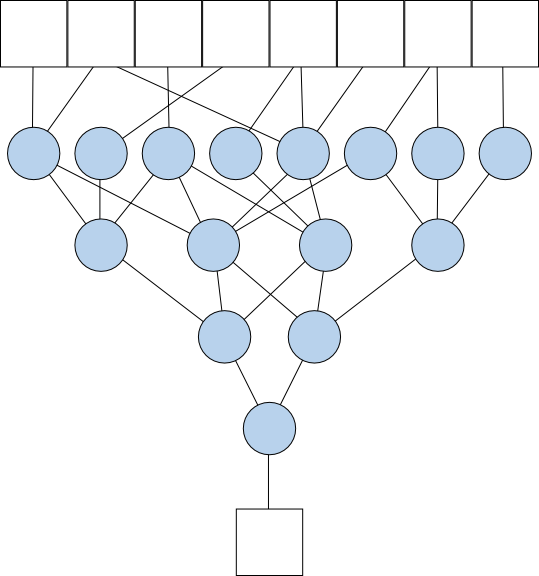
\includegraphics[width=.25\textwidth]{figures/specification}
	\caption{The figure we'd like to implement in TikZ.}
	\label{figure.worked-example.specification}
\end{figure}

As a first approximation, we may consider placing the nodes manually; though this seems unnecessarily laborious!
Listing \ref{listing.worked-example.1} illustrates how we might do this, and Figure \ref{figure.worked-example.1} shows how far I got before getting bored(!); we've also introduced the \texttt{scope} environment, this applies any options we give it to any Ti\emph{k}Z commands that fall within it.


\begin{figure}[btp]
	\centering
	\begin{subfigure}{.45\textwidth}
		\centering
		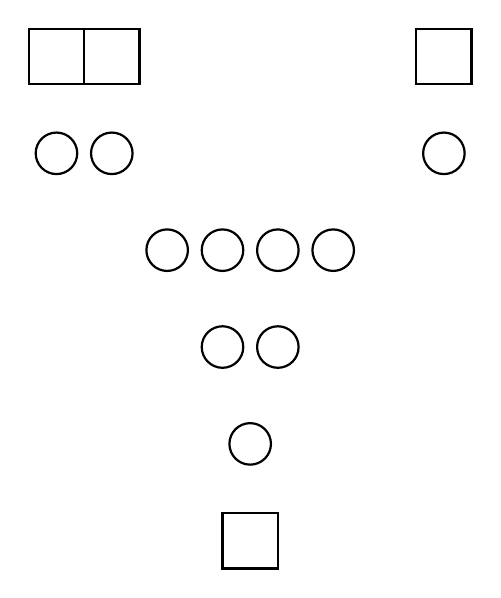
\begin{tikzpicture}

	%% The input row
	\begin{scope}[every node/.style={draw, thick, rectangle, minimum size=2em}]
		\node at ( 0em,0) (1-1) {};
		\node at ( 2em,0) (1-2) {};
		% ...
		\node at (14em,0) (1-8) {};
	\end{scope}

	%% The first row
	%% Shifted down (yshift=-...) and across (xshift=...)
	\begin{scope}[every node/.style={draw, thick, circle, minimum size=1.5em}, yshift=-3.5em]
		\node at ( 0em,0) (2-1) {};
		\node at ( 2em,0) (2-2) {};
		% ...
		\node at (14em,0) (2-8) {};
	\end{scope}

	%% The second row
	%% Shifted down (yshift=-...) and across (xshift=...)
	\begin{scope}[every node/.style={draw, thick, circle, minimum size=1.5em}, xshift=4em, yshift=-7.0em]
		\node at ( 0em,0) (3-1) {};
		\node at ( 2em,0) (3-2) {};
		\node at ( 4em,0) (3-3) {};
		\node at ( 6em,0) (3-4) {};
	\end{scope}

	%% The third row
	\begin{scope}[every node/.style={draw, thick, circle, minimum size=1.5em}, xshift=6em, yshift=-10.5em]
		\node at ( 0em,0) (4-1) {};
		\node at ( 2em,0) (4-2) {};
	\end{scope}

	%% The fourth row
	\begin{scope}[every node/.style={draw, thick, circle, minimum size=1.5em}, xshift=7em, yshift=-14.0em]
		\node at ( 0em,0) (5-1) {};
	\end{scope}

	%% The output row
	\begin{scope}[every node/.style={draw, thick, rectangle, minimum size=2em}, xshift=7em, yshift=-17.5em]
		\node at ( 0em,0) (6-1) {};
	\end{scope}

\end{tikzpicture}

		\caption{Manually placing nodes.}
		\label{figure.worked-example.1}
	\end{subfigure}
	\begin{subfigure}{.45\textwidth}
		\centering
		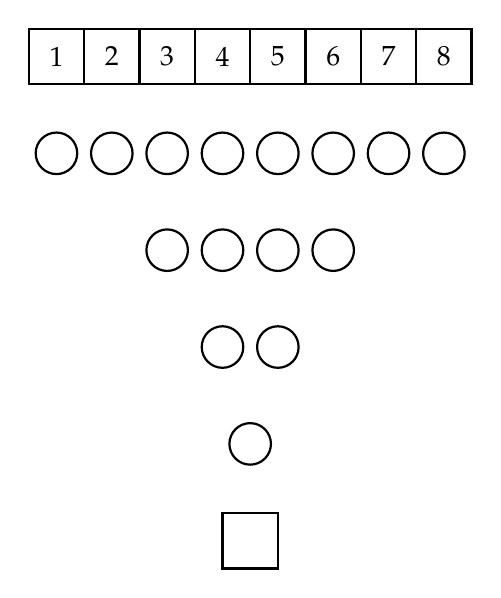
\begin{tikzpicture}

	%% The input row (index = 1)
	\begin{scope}[every node/.style={draw, thick, rectangle, minimum size=2em}]
		%% Iterate from 1-8, storing the index in \n
		\foreach \n in {1,...,8}{%
			\node at (\n*2em, 0) (1-\n) {\n};
		}
	\end{scope}

	%% Iterate through the processing rows
	%% We use a counter to track the row number
	\foreach [count=\r from 2] \m in {8, 4, 2, 1}{%
		%% Calculate the shifts using PGF math
		\pgfmathsetmacro\xShift{(8-\m)/2*2em}
		\pgfmathsetmacro\yShift{(\r-1)*-3.5em}

		\begin{scope}[every node/.style={draw, thick, circle, minimum size=1.5em}, xshift=\xShift, yshift=\yShift]
			\foreach \n in {1,...,\m}{%
				\node at (\n*2em, 0) (\r-\n) {};
			}
		\end{scope}
	}

	%% The output row
	\node at (9em,-17.5em) [draw, rectangle, thick, minimum size=2em] (6-1) {};

\end{tikzpicture}

		\caption{Using iteration to procedurally generate the nodes.}
		\label{figure.worked-example.2}
	\end{subfigure}
	\caption{Using TikZ to reproduce our target image.}
\end{figure}

\lstinputlisting[language=TeX, caption={Manual positioning of nodes.}, label={listing.worked-example.1}]{examples.article/worked-example-1.tex}

It should be obvious that there was a fair amount of unnecessary repetition when we place the nodes manually; thankfully by using PGF we can perform iteration.
The \texttt{\textbackslash foreach \textit{token} in \textit{list}\{\textit{action}\}} macro will perform \textit{action} for every item in the list.
Listing \ref{listing.worked-example.2} uses this to reduce the amount of work needed to produce the diagram, the result is shown in Figure \ref{figure.worked-example.2}.

\lstinputlisting[language=TeX, caption={Iterative positioning of nodes.}, label={listing.worked-example.2}]{examples.article/worked-example-2.tex}

This is far more concise, and would be an appropriate point to consider how to place edges.
First, however, we should note that our styles (\texttt{draw, rectangle, \ldots}) we spattered throughout our code, and it would be nice to refer to styles in terms of, say, \texttt{port} and \texttt{neuron}.
Thankfully, Ti\emph{k}Z also makes this possible!
The snippet of code shown in Listing \ref{listing.worked-example.3} creates two styles named as above, and means that we can replace lines 4 and 18 as below:\\
\texttt{\textbackslash begin\{scope\}[every node/.style=port, \ldots]}\\
\texttt{\textbackslash begin\{scope\}[every node/.style=neuron, \ldots]}

\lstinputlisting[language=TeX, caption={Creating our own styles.}, label={listing.worked-example.3}]{examples.article/worked-example-3.tex}

We should also note that we named our nodes by their row number, followed by a hyphen, followed by their number from left to right.
This will make it considerably easier to make connections between them.
Intuitively, all the code we need to link the 1st element of the 1st row with the 1st element of the 2nd row is:\\
\texttt{\textbackslash draw (1-1) to (2-1);}

Ideally, however, we would like a way of taking a list of pairs of the left-to-right number of the nodes to be connected, and then to add these arbitrary edges.
By extending the \texttt{foreach} command, this can be easily achieved.\\
\texttt{\textbackslash foreach \textbackslash x/\ldots/\textbackslash z in \{ 0/\ldots/n, \ldots \}\{\textit{actions\ldots}\}}

For example, the code in Listing \ref{listing.worked-example.4} will generate the links between the first two rows.

\lstinputlisting[language=TeX, caption={Automatically linking nodes using foreach.}, label={listing.worked-example.4}]{examples.article/worked-example-4.tex}

Even better, given a list of lists of pairs, we could generate all the links in one fell swoop; Listing \ref{listing.worked-example.5} illustrates this.

\lstinputlisting[language=TeX, caption={Automatically linking all nodes using foreach.}, label={listing.worked-example.5}]{examples.article/worked-example-5.tex}

Finally, putting all of the above together we get Listing \ref{listing.worked-example.finali}, the result of which is Figure \ref{figure.worked-example.final}.

\begin{figure}[btp]
	\begin{subfigure}{.5\textwidth}
		\centering
		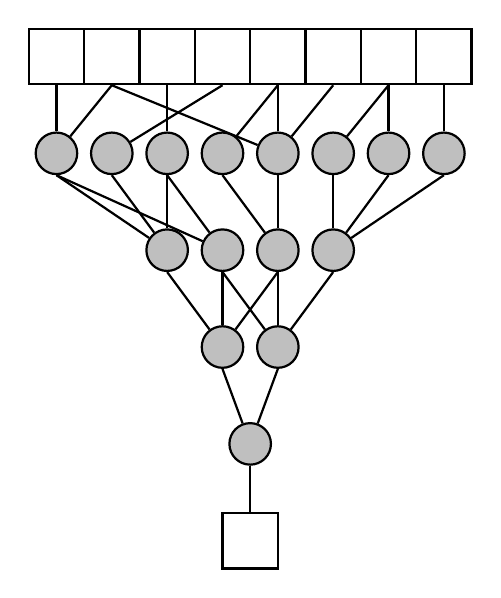
\begin{tikzpicture}[
	net node/.style = {draw, thick},
	port/.style = {net node, rectangle, minimum size=2em},
	neuron/.style = {net node, circle, minimum size=1.5em, fill=gray!50!white},
	edge/.style = {thick},
]

	%% The input row (index = 1)
	\begin{scope}
		%% Iterate from 1-8, storing the index in \n
		\foreach \n in {1,...,8}{%
			\node [port] at (\n*2em, 0) (1-\n) {};
		}
	\end{scope}

	%% Iterate through the processing rows
	%% We use a counter to track the row number
	\foreach [count=\r from 2] \m in {8, 4, 2, 1}{%
		%% Calculate the shifts using PGF math
		\pgfmathsetmacro\xShift{(8-\m)/2*2em}
		\pgfmathsetmacro\yShift{(\r-1)*-3.5em}

		\begin{scope}[xshift=\xShift, yshift=\yShift]
			\foreach \n in {1,...,\m}{%
				\node [neuron] at (\n*2em, 0) (\r-\n) {};
			}
		\end{scope}
	}

	%% The output row
	\node at (9em,-17.5em) [port] (6-1) {};

	%% Draw the connections
	%% User specified
	\foreach [count=\m] \l in {%
		{1/1, 2/1, 2/5, 3/3, 4/2, 5/4, 5/5, 6/5, 7/6, 7/7, 8/8},	% 1st to 2nd
		{1/1, 1/2, 2/1, 3/1, 3/2, 4/3, 5/3, 6/4, 7/4, 8/4},		% 2nd to 3rd
		{1/1, 2/1, 2/2, 3/1, 3/2, 4/2},					% 3rd to 4th
	}{%
		%% \m is the start row, let \n be the end row
		\pgfmathtruncatemacro\n{\m+1}	% Truncate makes an int from a float
	
		\foreach \u/\v in \l {% Here \l is one of the lists defined above
			\draw [edge] (\m-\u.south) to (\n-\v);
		}
	}

	%% Always present
	\foreach [count=\m from 4] \l in {{1/1, 2/1}, {1/1}}{%
		\pgfmathtruncatemacro\n{\m+1}	% Truncate makes an int from a float
		\foreach \u/\v in \l {% Here \l is one of the lists defined above
			\draw [edge] (\m-\u.south) to (\n-\v);
		}
	}

\end{tikzpicture}

		\caption{The final result, not quite as specified, but certainly close enough, and easily reused.}
		\label{figure.worked-example.final}
	\end{subfigure}
	\begin{subfigure}{.5\textwidth}
		\centering
		\newcommand*{\neuralnetdiagram}[1]{% A new command called \neuralnetdiagram with 1 parameter `#1'
\begin{tikzpicture}[
	net node/.style = {draw, thick},
	port/.style = {net node, rectangle, minimum size=2em},
	neuron/.style = {net node, circle, minimum size=1.5em, fill=gray!50!white},
	edge/.style = {thick},
]

	%% The input row (index = 1)
	\begin{scope}
		%% Iterate from 1-8, storing the index in \n
		\foreach \n in {1,...,8}{%
			\node [port] at (\n*2em, 0) (1-\n) {};
		}
	\end{scope}

	%% Iterate through the processing rows
	%% We use a counter to track the row number
	\foreach [count=\r from 2] \m in {8, 4, 2, 1}{%
		%% Calculate the shifts using PGF math
		\pgfmathsetmacro\xShift{(8-\m)/2*2em}
		\pgfmathsetmacro\yShift{(\r-1)*-3.5em}

		\begin{scope}[xshift=\xShift, yshift=\yShift]
			\foreach \n in {1,...,\m}{%
				\node [neuron] at (\n*2em, 0) (\r-\n) {};
			}
		\end{scope}
	}

	%% The output row
	\node at (9em,-17.5em) [port] (6-1) {};

	%% Draw the connections
	%% User specified
	\foreach [count=\m] \l in {#1}{% This uses our parameter
		%% \m is the start row, let \n be the end row
		\pgfmathtruncatemacro\n{\m+1}	% Truncate makes an int from a float
	
		\foreach \u/\v in \l {% Here \l is one of the lists defined above
			\draw [edge] (\m-\u.south) to (\n-\v);
		}
	}

	%% Always present
	\foreach [count=\m from 4] \l in {{1/1, 2/1}, {1/1}}{%
		\pgfmathtruncatemacro\n{\m+1}	% Truncate makes an int from a float
		\foreach \u/\v in \l {% Here \l is one of the lists defined above
			\draw [edge] (\m-\u.south) to (\n-\v);
		}
	}

\end{tikzpicture}
}

		\neuralnetdiagram{%
			{1/1, 1/2, 2/1, 2/3, 3/3, 3/4, 4/4, 5/5, 6/6, 8/6, 8/7, 8/8},%
			{1/1, 2/1, 3/1, 3/2, 4/2, 5/4, 6/3, 6/4, 7/3, 8/4},%
			{1/1, 2/1, 3/2, 4/2},%
		}
		\caption{The result of the macro to generate a different network connectivity.}
	\end{subfigure}
	\caption{The results of our labours.}
\end{figure}

Having mentioned reuse as desirable, a good question is, can we wrap this in a macro that accepts the list of connections as a parameter and then draws the network?
The answer, unsurprisingly, is \textit{yes}.
Listing \ref{listing.worked-example.finalii} shows how we'd modify the code to make a macro, and then we can draw the diagram with \texttt{\textbackslash neuralnetdiagram\{\textit{list}\}}.

\lstinputlisting[language=TeX, caption={The final result.}, label={listing.worked-example.finali}]{examples.article/worked-example-finali.tex}
\lstinputlisting[language=TeX, caption={The final result, modified to produce a parametrised macro.}, label={listing.worked-example.finalii}]{examples.article/worked-example-finalii.tex}

\mode<all>	%% Reset mode again

		\appendix
		\section{Some Further Examples}
\subsection{Animating a Diagram -- Free Body Projection}

\mode<presentation>
\begin{frame}[label=projection]
	\frametitle{Animating a Diagram -- Free Body Projection}
	\begin{center}
		%% Free Body Projection Diagram for Beamer
%% ---------------------------------------
%% (C) Andrew Mundy 2013
%%
%% Shows the displacement and velocity of a particle
%% projected with given initial velocity and displacement
%% from time t=0 until the last integral time before the
%% particle would hit the ground.
%%
%% Usage:
%% Just place in a Beamer frame.

\begin{tikzpicture}[
	xscale=0.25,
	yscale=0.20,
	ball/.style = {circle, fill=uomgrey!50!white},
	vector/.style = {thick, ->, uomgrey!50!white},
	current ball/.style = {ball, fill=blue},
	current vector/.style = {vector, blue},
	every label/.style = {font=\tiny},
]
	%% Set the initial velocity
	\def\ui{5}
	\def\uj{15}

	%% Set the initial position
	\def\si{0}
	\def\sj{0}

	%% Set the acceleration
	\def\ai{0}
	\def\aj{-9.8}

	%% Determine the point when we reach the ground, and round down for the last integral
	%% time interval to show.
	\pgfmathsetmacro\groundt{-(2*\uj)/\aj}
	\pgfmathtruncatemacro\maxt{floor(\groundt)}
	\pgfmathsetmacro\maxsi{\si + \ui*\groundt + (\ai*\groundt*\groundt)/2}

	%% Some PGF Configuration
	%% Prints floats with up to 2d.p.
	\pgfkeys{/pgf/number format/.cd,fixed,precision=2}

	%% Draw the ground
	\draw (0,0) -- (\maxsi, 0);
	\fill [pattern=north west lines, pattern color=gray] (0,0) rectangle (\maxsi, -5em);

	%% Now display the ball for times 0, 1, ..., \maxt
	\foreach [count=\c] \t in {0,...,\maxt}{%
		%% Determine the current position
		%% s = ut + 1/2at^2
		\pgfmathsetmacro\sti{\si + \ui*\t + (\ai*\t*\t)/2}
		\pgfmathsetmacro\stj{\sj + \uj*\t + (\aj*\t*\t)/2}

		%% Determine the current velocity
		\pgfmathsetmacro\vti{\ui + \ai*\t}
		\pgfmathsetmacro\vtj{\uj + \aj*\t}

		%% Convert the velocity to polar co-ordinates
		%% [1] Strictly not necessary, but cool
		\pgfmathsetmacro\argvt{atan( \vtj / \vti )}
		\pgfmathsetmacro\magvt{sqrt( \vti*\vti + \vtj*\vtj )}

		%% Save the ball's position as a co-ordinate
		\coordinate (ball-at-\t) at (\sti, \stj);

		%% Draw the ball (shadow/past)
		\pgfmathtruncatemacro\ci{\c + 1}
		\visible<\ci->{
			\node at (ball-at-\t) [ball] {};
			\draw [vector] (ball-at-\t.center) -- ++(\argvt:\magvt);
			%% Would have worked equally well (and saved us [1] above)
			% \draw [vector] (ball-at-\t.center) -- ++(\vti,\vtj);
		}

		%% Draw the ball
		\visible<\c>{ 
			\node at (ball-at-\t) [
				current ball,
				label={left:{$\vec{v}(\t) = \pgfmathprintnumber{\vti}\vec{i} +%
						\pgfmathprintnumber{\vtj}\vec{j}$}},
			] {};
			\draw [current vector] (ball-at-\t.center) -- ++(\argvt:\magvt);
			%% Would have worked equally well
			% \draw [current vector] (ball-at-\t.center) -- ++(\vti,\vtj);
		}
	}
\end{tikzpicture}

	\end{center}
\end{frame}
\mode*

Ti\emph{k}Z integrates well with Beamer (they were created by the same person) -- the code in Listing \ref{listing.examples.projection} shows the motion of a projected particle at time intervals of one second, output in Figure \ref{figure.examples.projection}.

\begin{figure}[!Btp]
	\centering
	\foreach \n in {1,...,4}{%
		\begin{subfigure}{.225\textwidth}
			\includeslide[width=\textwidth]{projection<\n>}
		\end{subfigure}
	}
	\caption{Animated free body projection using TikZ and Beamer}
	\label{figure.examples.projection}
\end{figure}

\lstinputlisting[language=TeX, caption={Animating a free body projection with TikZ and Beamer.}, label={listing.examples.projection}]{examples.beamer/projection}

\subsection{Petri Nets}

\mode<presentation>
\begin{frame}[label=petri]
	\frametitle{Petri Nets, Illustrating Chains and Matrices}
	\begin{center}
		%% Simple Petri Net Model
%% ----------------------
%% (C) Andrew Mundy 2013
%% 
%% Displays a simple Petri net and then evolves the markings.
%% 
%% Requirements
%% ------------
%% \usepackage{tikz}
%% \usetikzlibrary{automata, chains, petri, matrices, scopes}

\begin{tikzpicture}[
	petri node/.style = {minimum size=1em},
	petri join/.style = {very thick, ->, shorten >= 1pt},
%
	place/.style = {petri node, circle, draw, very thick},
	transition/.style = {petri node, rectangle, fill},
%
	every join/.style = {petri join},
	every matrix/.style = {row sep = 1em, column sep = 2em},
	every token/.style = {fill=contentgray},	%% Remove this line if you get an error
]

	%% Draw the Petri Net
	%% Using a matrix for node placement, the & character signifies a new column, and \\ a new row.
	\matrix [] {
		\node [place] (p1) {}; & & \node [place] (p2) {};	\\
		\node [transition, label=left:$a$] (a) {}; & & \node [transition, label=right:$b$] (b) {};	\\
		\node [place] (p3) {}; & & \node [place] (p4) {};	\\
		& \node [transition, label=below:$c$] (c) {};			\\
	};

	%% Here create a chain, and use the \chainin command to add pre-existing nodes
	%% The join option draws the join between one node and the previous.
	{ [start chain=thr1]
		\chainin (p1);
		\chainin (a) [join];
		\chainin (p3) [join];
		\chainin (c) [join=by {petri join, bend right}];
		\chainin (p1) [join=by {petri join, out=90, in=0}];
	}

	{ [start chain=thr2]
		\chainin (p2);
		\chainin (b) [join];
		\chainin (p4) [join];
		\chainin (c) [join=by {petri join, bend left}];
		\chainin (p2) [join=by {petri join, out=90, in=180}];
	}

	%% Draw the markings
	%% Each marking is a list of places with a token present
	\foreach [count=\c from 1] \marking in {%
		{1,2},		   % Initial Marking
		{3,2},		   % a fired
		{3,4},		   % b fired
		{1,2},		   % c fired
		{1,4},		   % b fired
		{3,4},		   % a fired
		{1,2}%
	}{%
		\only<\c>{%
			\foreach \place in \marking {%
				\node [token] at (p\place) {};
			}
		}
	}
\end{tikzpicture}

	\end{center}
\end{frame}
\mode*

This example introduces two exceptionally important libraries that we sadly didn't have time for in the talk, \textbf{matrices} and \texttt{chains}.
As expected, matrices allow for grid like placing of nodes; and chains are a semantic method for joining groups on nodes up.
The Petri Net example shown in Listing \ref{listing.examples.petri} is animated for Beamer (in that it transitions through several markings), and the first slide is shown in Figure \ref{figure.examples.petri}.

\begin{figure}[btp]
	\centering
	\includeslide[width=.5\textwidth]{petri}
	\caption{Petri Nets in TikZ}
	\label{figure.examples.petri}
\end{figure}

\lstinputlisting[language=TeX, caption={An animated Petri Net.}, label={listing.examples.petri}]{examples.beamer/petri}

\subsection{Vector Fields (Charged Particles)}

\mode<presentation>
\begin{frame}
	\frametitle{Vector Fields (Charged Particles)}
	\begin{center}
		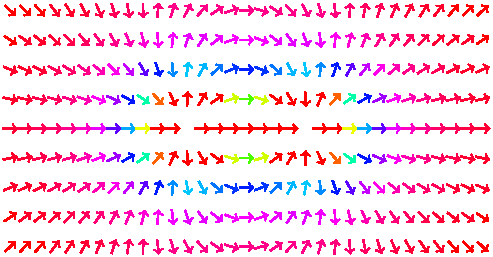
\includegraphics{examples.beamer/field-crop}
	\end{center}
\end{frame}
\mode*

Hopefully, this should be of interest, but mostly as an example of something that is not particularly efficient in Ti\emph{k}Z.
Essentially, the code, in Listing \ref{listing.examples.field}, models the electric field due to several charged particles in 2D space, the resulting graphic uses hue to represent field strength and an arrow to illustrate field direction, as in Figure \ref{figure.examples.fields}.

\begin{figure}[btp]
	\centering
	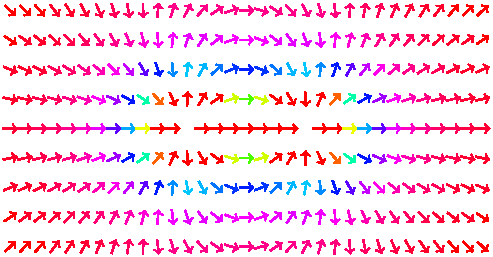
\includegraphics{examples.beamer/field-crop}
	\caption{Computing and illustrating vector fields using TikZ and PGF}
	\label{figure.examples.fields}
\end{figure}

\lstinputlisting[language=TeX, caption={Illustrating a vector field using TikZ and PGF.}, label={listing.examples.field}]{examples.beamer/field}

	\mode*

	\begin{frame}
		\frametitle{Useful Resources}
		\begin{itemize}
			\item \url{http://texample.net} -- Examples
			\item The PGF Manual (Sourceforge)
		\end{itemize}

		\begin{description}
			\item[Slides] \url{http://amundy.co.uk/documents/tikzbox.beamer.pdf}
			\item[Handout] \url{http://amundy.co.uk/documents/tikzbox.article.pdf}
			\item[Sources] \url{https://github.com/AndrewMundy/tikz-box}
		\end{description}
	\end{frame}
\end{document}

